%============================================================
% Forward Model diagram
% Required images (place in tikz/images/):
%   pk_linear.png        — linear matter power spectrum P_L(k) curve
%   delta_ic_cube.png    — linear initial-conditions density cube
%   delta_fin_cube.png   — evolved dark-matter density cube
%   delta_biased_cube.png— evolved biased-tracer density cube
%   posterior_corner.png — inferred posterior corner plot
% (Layout smoke-test: \usepackage{mwe} and replace each path with example-image)
%============================================================
\documentclass[tikz, border=2mm]{standalone}
\usepackage{tikz}
\usepackage{amsmath}
\usepackage{amssymb}
\usepackage{bm}
\usetikzlibrary{shapes.geometric, positioning, arrows.meta, calc}
\usepackage[dvipsnames]{xcolor}

% --- Overleaf guard ---------------------------------------------------------
% Overleaf compiles every file with jobname "output", shared with main.tex.
% Without this, the figure reads main.tex's biblatex "output.aux" at
% \begin{document} and dies on \abx@aux@cite / \abx@aux@refcontext etc.
% This figure has no \cite/\ref, so we simply skip that .aux read.
\makeatletter\let\@input\@gobble\makeatother
% ---------------------------------------------------------------------------

\begin{document}
% Uniformly rescale the finished figure to fit an A4 text block (here 15.4cm x
% 24.7cm for top/bottom=2.5cm, left/right=2.8cm margins), leaving room for a
% caption. \resizebox scales everything -- nodes, text, line widths and the
% embedded \includegraphics images -- together, so nothing is distorted.
% Change "22cm" to taste (the width follows automatically from the aspect ratio).
\resizebox{!}{22cm}{
    \begin{tikzpicture}[
        >=Stealth,
        font=\large,
        % stretch the layout vertically so the connecting arrows have more room.
        % yscale moves node *positions* (and the path-drawn panel) apart while
        % node sizes, text and \includegraphics widths stay fixed -> no distortion.
        yscale=1.3,
        % operation boxes
        op/.style={rectangle, draw=MidnightBlue!65, rounded corners, fill=MidnightBlue,
                   fill opacity=0.13, text opacity=1, align=center,
                   minimum height=1.0cm, inner sep=6pt},
        % prior / input box
        inp/.style={op, draw=gray, fill=Gray, fill opacity=0.20},
        % side / auxiliary output box (dashed to mark it as a branch off the main flow)
        aux/.style={op, draw=gray, dashed, fill=Gray, fill opacity=0.10},
        lbl/.style={black, scale=0.82, align=center},
        note/.style={black!55, scale=0.62, align=center},
        stage/.style={gray!75, scale=0.78, font=\scshape, rotate=90, align=center},
        arr/.style={->, line width=0.9pt, rounded corners=3pt, black!72},
        bus/.style={line width=0.9pt, black!72},
        lead/.style={densely dotted, line width=0.6pt, gray},
        junc/.style={circle, fill=black!72, inner sep=1.7pt}
    ]
    
    % ---- column axes (symmetric about the centre spine) ------------------
    \def\xc{7.0}      % centre spine
    \def\xL{4.2}      % left tracer lane
    \def\xR{9.8}      % right tracer lane
    \def\xF{13.0}     % Fisher side branch
    \def\xS{11.2}     % top-right P_L(k) inset
    
    % =====================================================================
    % Outer panel + title
    % =====================================================================
    \draw[MidnightBlue!55, rounded corners, fill=MidnightBlue, fill opacity=0.05]
          (0.3,-5.6) rectangle (14.9,13.0);
    \node[draw=MidnightBlue, fill=MidnightBlue, fill opacity=1, rounded corners,
          text=white, minimum width=4.4cm, minimum height=0.85cm, font=\large\bfseries]
          at (\xc, 13.0) {Forward Model};
    
    % ---- faint stage labels down the left margin ------------------------
    \node[stage] at (0.85, 9.3)  {initial conditions};
    \node[stage] at (0.85, 6.9)  {gravity};
    \node[stage] at (0.85, 4.4)  {final fields};
    \node[stage] at (0.85, 0.9)  {compression};
    \node[stage] at (0.85,-2.6)  {inference};
    
    % =====================================================================
    % (1) Cosmology  ->  initial conditions   (centre spine, flows down)
    % =====================================================================
    \node[inp] (theta) at (\xc, 11.6)
       {From prior: $\bm{\theta}$};
    
    \node[op] (pk) at (\xc, 10.1) {Linear $P_L(k)$\\[1pt]\footnotesize DiscoDJ};
    
    % P_L(k) preview, parked top-right and tied to its box with a dotted leader
    % \node[draw=gray, rounded corners, inner sep=2pt, fill=white] (pkimg) at (\xS, 10.1)
    %    {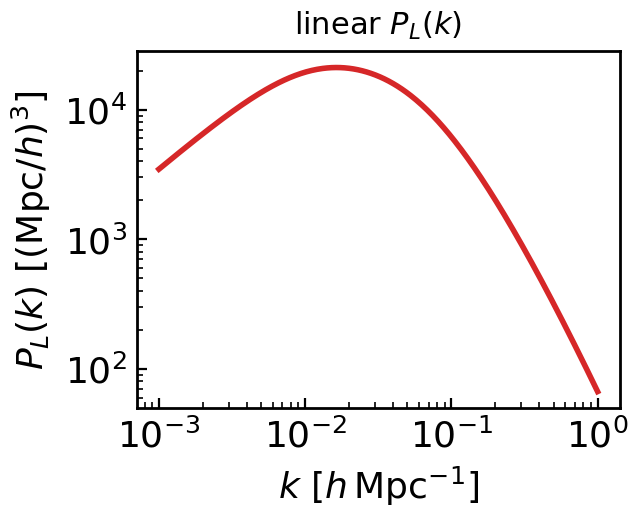
\includegraphics[width=2.0cm]{images/pk_linear.png}};
    % \node[note] at (\xS, 8.95) {$P_L(k)$};
    % \draw[lead] (pk.east) -- (pkimg.west);
    
    \node (dic) at (\xc, 8.5) {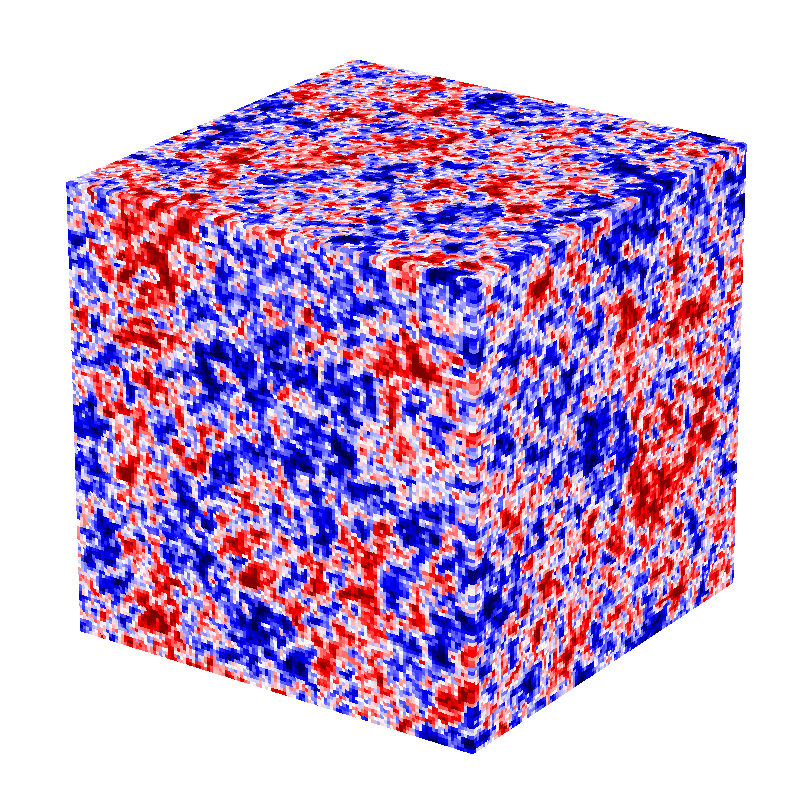
\includegraphics[width=1.6cm]{images/delta_ic_cube.png}};
    \node[lbl, anchor=west] at (8.05, 8.65) {$\bm{\delta}_{\rm ic}$\\[1pt]initial conditions};
    
    \node[op, minimum width=3.6cm] (nbody) at (\xc, 6.9) {2LPT $+$ PM};
    
    \draw[arr] (theta.south) -- (pk.north);
    \draw[arr] (pk.south)  -- (dic.north);
    \draw[arr] (dic.south)  -- (nbody.north);

    % =====================================================================
    % (2) Tracer branches   (symmetric fork into two lanes)
    % =====================================================================
    \node[op, minimum width=3.0cm] (scat) at (\xL, 5.3)
       {scatter\\[1pt]\footnotesize uniform weights $=1$};
    \node[op, minimum width=3.4cm, inner sep=4pt, font=\small] (bias) at
  (\xR, 5.3)
     {Lagrangian bias $w(\bm{q})$\\[1pt]

  \scriptsize$1+b_1\delta+b_2(\delta^2{-}\langle\delta^2\rangle)$\\[-1pt]
      \scriptsize$+\,b_{s^2}(s^2{-}\langle
  s^2\rangle)+b_{n^2}\nabla^2\delta$};
    
    \coordinate (fork) at (\xc, 6.1);
    \draw[arr] (nbody.south) -- (fork) -| (scat.north);
    \draw[arr] (fork) -| (bias.north);
    
    % --- tracer density fields
    \node (dfin)  at (\xL, 3.6) {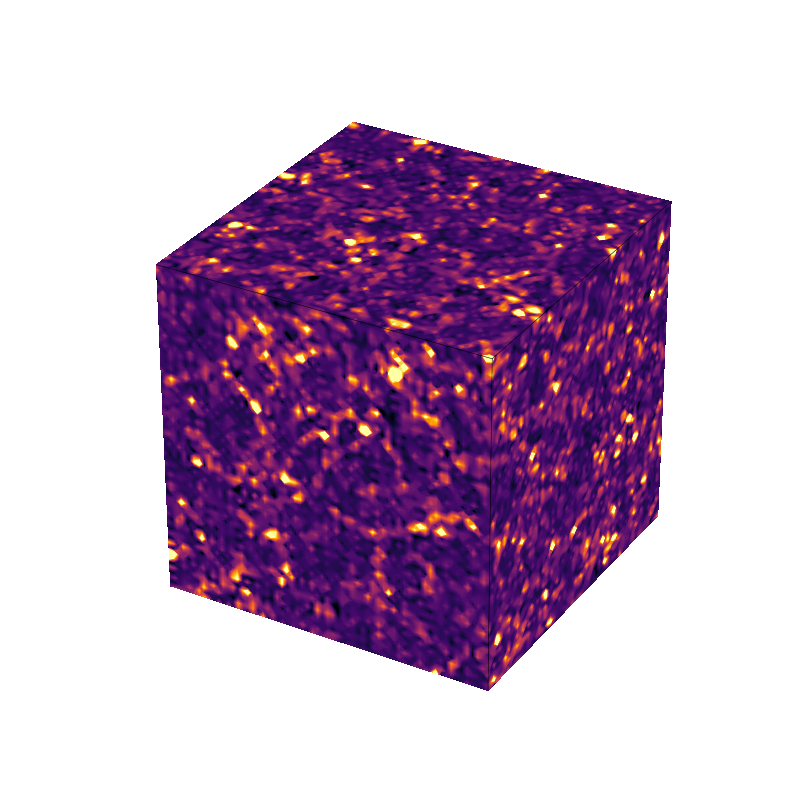
\includegraphics[width=1.7cm]{images/delta_fin_cube.png}};
    \node (dbias) at (\xR, 3.6) {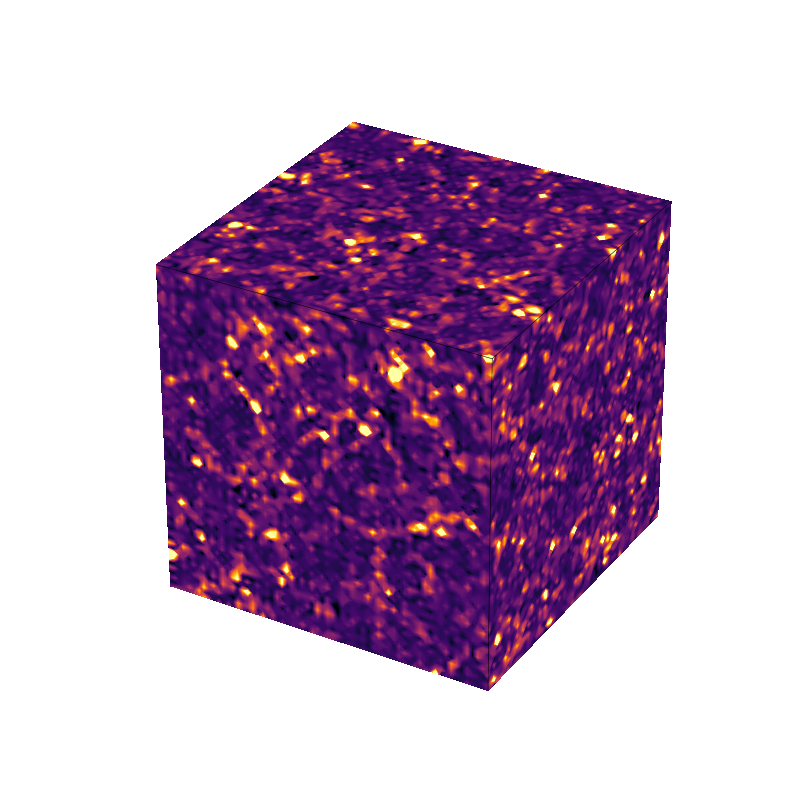
\includegraphics[width=1.7cm]{images/delta_biased_cube.png}};
    \node[lbl, anchor=east] at (\xL-0.55, 3.6) {$\bm{\delta}_{\rm dm}$\\[1pt]dark matter};
    \node[lbl, anchor=west] at (\xR+1.15, 3.6) {$\bm{\delta}_{\rm g}$\\[1pt]biased tracer};
    \draw[arr] (scat.south) -- (dfin.north);
    \draw[arr] (bias.south) -- (dbias.north);
    
    % =====================================================================
    % (3) Summaries  --  a shared bus so both fields feed both summaries
    %     (horizontal rail instead of a 2x2 criss-cross)
    % =====================================================================
    \node[op, minimum width=3.0cm] (cnn) at (\xL, 1.4)
       {Field compression\\[1pt]\footnotesize CNN / ViT};
    \node[op, minimum width=3.8cm] (bfast) at (\xR, 1.4)
       {BFast\\[1pt]\footnotesize$P_{0,2,4}(k)+B_0(k_1,k_2,k_3)$};
    
    % straight lane stems ...
    \draw[arr] (dfin.south)  -- (cnn.north);
    \draw[arr] (dbias.south) -- (bfast.north);
    % ... linked by a horizontal bus (both fields available to both summaries)
    \draw[bus] (\xL,2.5) -- (\xR,2.5);
    \node[junc] at (\xL,2.5) {};
    \node[junc] at (\xR,2.5) {};
    
    % =====================================================================
    % (4) Inference   (symmetric funnel into SBI, then the posterior)
    % =====================================================================
    \node[aux, minimum width=3.4cm] (scomp) at (\xR, -0.3)
       {Summary compression\\[1pt]\footnotesize none / MLP / PCA};
    \node[aux, minimum width=2.2cm] (fisher) at (13.6, 1.4) {Fisher\\forecast};
    \node[op, minimum width=2.0cm] (sbi) at (\xc, -2.3) {SBI};
    \node (post) at (\xc, -4.1) {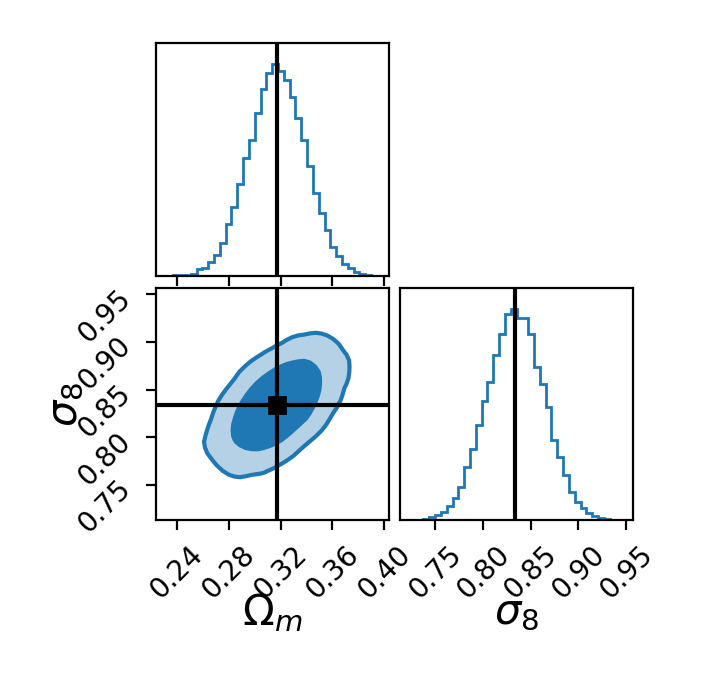
\includegraphics[width=2.1cm]{images/posterior_corner.png}};
    \node[lbl] at (\xc, -5.3) {posterior $p(\bm{\theta}\,|\,\bm{d})$};
    
    % BFast -> summary compression (down) and -> Fisher forecast (side branch)
    \draw[arr] (bfast.south) -- (scomp.north);
    \draw[arr] (bfast.east) -- (fisher.west) ;
    % field compression + compressed summaries funnel into SBI -> posterior
    \coordinate (sbimerge) at (\xc, -1.45);
    \draw[bus] (cnn.south)   |- (sbimerge);
    \draw[bus] (scomp.south) |- (sbimerge);
    \node[junc] at (sbimerge) {};
    \draw[arr] (sbimerge) -- (sbi.north);
    \draw[arr] (sbi.south) -- (post.north);
    
    \end{tikzpicture}}% end \resizebox
\end{document}
